\section{研究相关理论}

\subsection{排队论}
排队是在日常生活中经常遇到的现象,如顾客到商店购买物品、病人到医院看病常常
要排队。此时要求服务的人数超过服务机构的容量,即到达
的顾客不能立即得到服务,因而出现了排队现象。这种现象不仅在个人日常生活中出现,
电话局的占线问题,车站、码头等交通枢纽的车船堵塞和疏导,故障机器的停机待修,,水库
水量的存储调节等都是有形或无形的排队现象。由
于顾客到达和服务时间的随机性,可以说排队现象几乎是不可避免的。
如果增添服务设备,就要增加投资或发生空闲浪费;如果服务设备太少,排队现象就
会严重,对顾客个人和对社会都会带来不利影响。因此,管理人员必须考虑如何在这两者
之间取得平衡,经常检查目前处理是否得当,研究今后改进对策,以期提高服务质量,降低
成本\cite{ycx}。

排队模型常表示成 $X/Y/Z/A/B/C$ (相继到达的间隔时间/服务时间的分布/服务台的数目/容量限制/客源数目/服务规则)形式,
对于一个公交站台可以表示成标准的 $M/M/1$ 模型,该系统的特点:

(1)输入过程———顾客源是无限的,顾客单个到来,相互独立,一定时间的到达数服
从泊松分布,到达过程已是平稳的。

(2)排队规则———单队,且对队长没有限制,先到先服务。

(3)服务机构———单服务台,各顾客的服务时间是相互独立的,服从相同的负指数
分布。

此外,还假定到达间隔时间和服务时间是相互独立的。

已知 $M/M/1$ 模型到达规律服从参数为 $\lambda$ 的泊松分布,服务时间服从参数为 $\mu$ 的负指数分布,
给出 $t$ 时刻状态为 $n$ (系统中有 $n$ 个顾客)的概率 $P_{n}(t)$,系统的状态方程可以表示为:
\begin{equation}\label{fomula1}
    \begin{cases}
        -\lambda P_0 + \mu P_1 = 0
        \\
       \lambda p_{n - 1} + \mu P_{n + 1} - (\lambda + \mu)P_n = 0 \qquad n\ge 1
       \end{cases}
\end{equation}

式~\ref{fomula1}~是关于 $P_{n}$ 的差分方程,它表明的各状态之间的转移关系如图~\ref{fig21}~所示。

\begin{figure}[h]
\centering
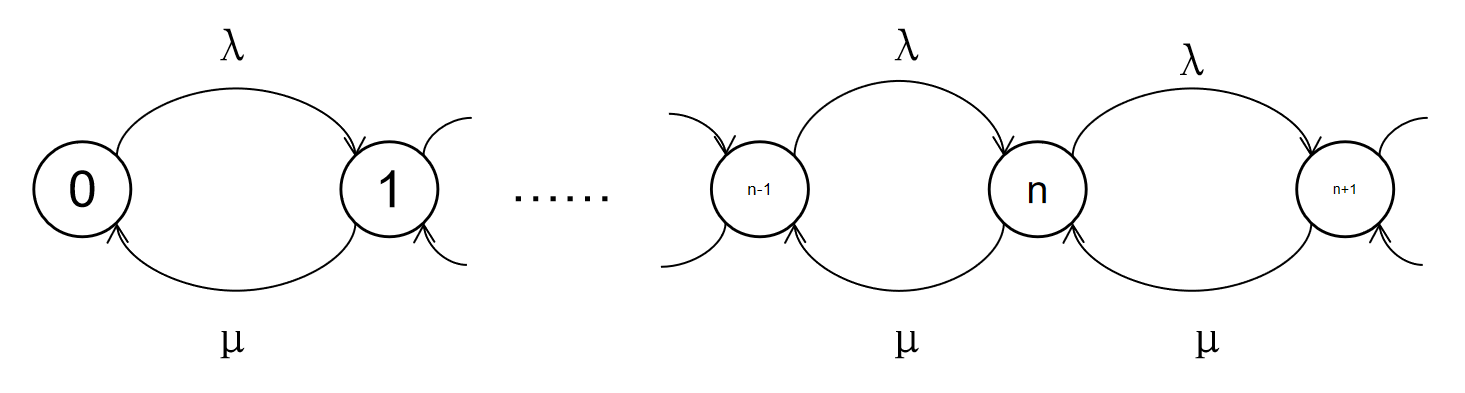
\includegraphics[width=0.80\textwidth]{figs/chap02/fig21.png}
\caption{M/M/1模型状态转移示意图}
\label{fig21}
\end{figure}